\section{Metodología, Desarrollo y Validación}
\label{sec:metodologia}

En esta sección se expone de forma pormenorizada el procedimiento metodológico implementado para transformar los microdatos brutos de la EAIMCS 2017--2018 en un sistema predictivo robusto, insesgado y validado empíricamente.

\subsection{Pipeline de Preprocesamiento e Ingeniería de Datos}
El procesamiento de los microdatos se organizó en un pipeline modular y determinista compuesto por cinco etapas secuenciales, cuya trazabilidad se registra formalmente en el artefacto inmutable \texttt{bitacora\_preprocesamiento.json}:

\begin{enumerate}
    \item \textbf{Tratamiento de Valores Centinela (\texttt{99999.0}):}
    En la base original del INE, el valor numérico \texttt{99999.0} no representa una magnitud monetaria real, sino una convención estadística para señalar registros con imputación pendiente o inconsistencia contable. Todos los valores centinela fueron transformados sistemáticamente a valores nulos (\texttt{NaN}), y los montos monetarios anómalos menores a cero fueron acotados mediante la función $\max(0, x)$.
    
    \item \textbf{Agregación Relacional de la Sección 10 (Materias Primas):}
    El módulo de materiales (\texttt{MOD\_ANUAL\_S10}) presenta una estructura tabular desagregada (6,428 filas correspondientes a múltiples insumos por empresa). Se aplicó una agregación relacional a nivel del identificador único \texttt{ID}, reduciendo el conjunto a 1,614 empresas mediante tres variables sintéticas:
    \begin{itemize}
        \item Diversidad de insumos utilizados: $n\_insumos$.
        \item Gasto total anual en compras de materiales: $total\_valor\_co$.
        \item Consumo total fabril de materias primas: $total\_valor\_uti$.
    \end{itemize}
    Para aquellas empresas pertenecientes a sectores de comercio o servicios puros sin reporte en la Sección 10, dichos campos fueron imputados a cero mediante un cruce por la izquierda (\textit{Left Join}).

    \item \textbf{Normalización Categórica CAEB y Departamentos:}
    Los 445 códigos de actividad económica desagregada a 4 dígitos de la Clasificación de Actividades Económicas de Bolivia (CAEB, basada en la CIIU Rev. 4) fueron agrupados en 14 macrosectores homogéneos (Industria Textil, Alimentos y Bebidas, Comercio Mayorista, Construcción, etc.). Asimismo, se codificaron los 9 departamentos del país.

    \item \textbf{Blindaje Metodológico Anti-Fuga de Datos (\textit{Anti-Leakage}):}
    Se implementó una política explícita de exclusión que descartó 19 variables calculadas con posterioridad a la encuesta por los economistas de Cuentas Nacionales (como el Valor Bruto de Producción, Valor Agregado Bruto, Consumo Intermedio) y los componentes de ingresos directos de la Sección 5 (\texttt{S05\_01} a \texttt{S05\_04}). Esto garantiza que el modelo aprenda exclusivamente a partir de la capacidad productiva instalada.

    \item \textbf{Transformación Logarítmica No Lineal:}
    Dada la severa asimetría positiva de los datos económicos (asimetría de cola pesada), se aplicó la transformación monótona $\ln(1 + x)$ a los 11 predictores cuantitativos y a la variable objetivo:
    \begin{equation}
        y_{\log} = \ln(y + 1), \quad X_{\log, j} = \ln(X_j + 1)
        \label{eq:log1p}
    \end{equation}
    Esta transformación estabiliza la varianza de los residuos y aproxima la distribución de errores a una forma cuasi-normal homocedástica, como se ilustra en la Figura \ref{fig:distribucion_asimetria_log}.
\end{enumerate}

En la Figura \ref{fig:pipeline_linaje_datos} se expone el diagrama arquitectónico formal que representa el linaje integral de los datos, ilustrando la ingestión dual desde el perímetro de almacenamiento crudo del INE (Dataset Primario general y Dataset Secundario de insumos), los procesos de saneamiento y agregación relacional $N \rightarrow 1$, el ensamble \textit{Left Join}, el blindaje metodológico anti-fuga de datos y la partición estratificada consumida por el sistema de auditoría.

\begin{figure}[htbp]
\centering
\caption{Arquitectura de Integración de Datos: Ingestión Dual (Dataset Primario y Secundario), Pipeline de Transformación y Flujo de Consumo Predictivo.}
\label{fig:pipeline_linaje_datos}
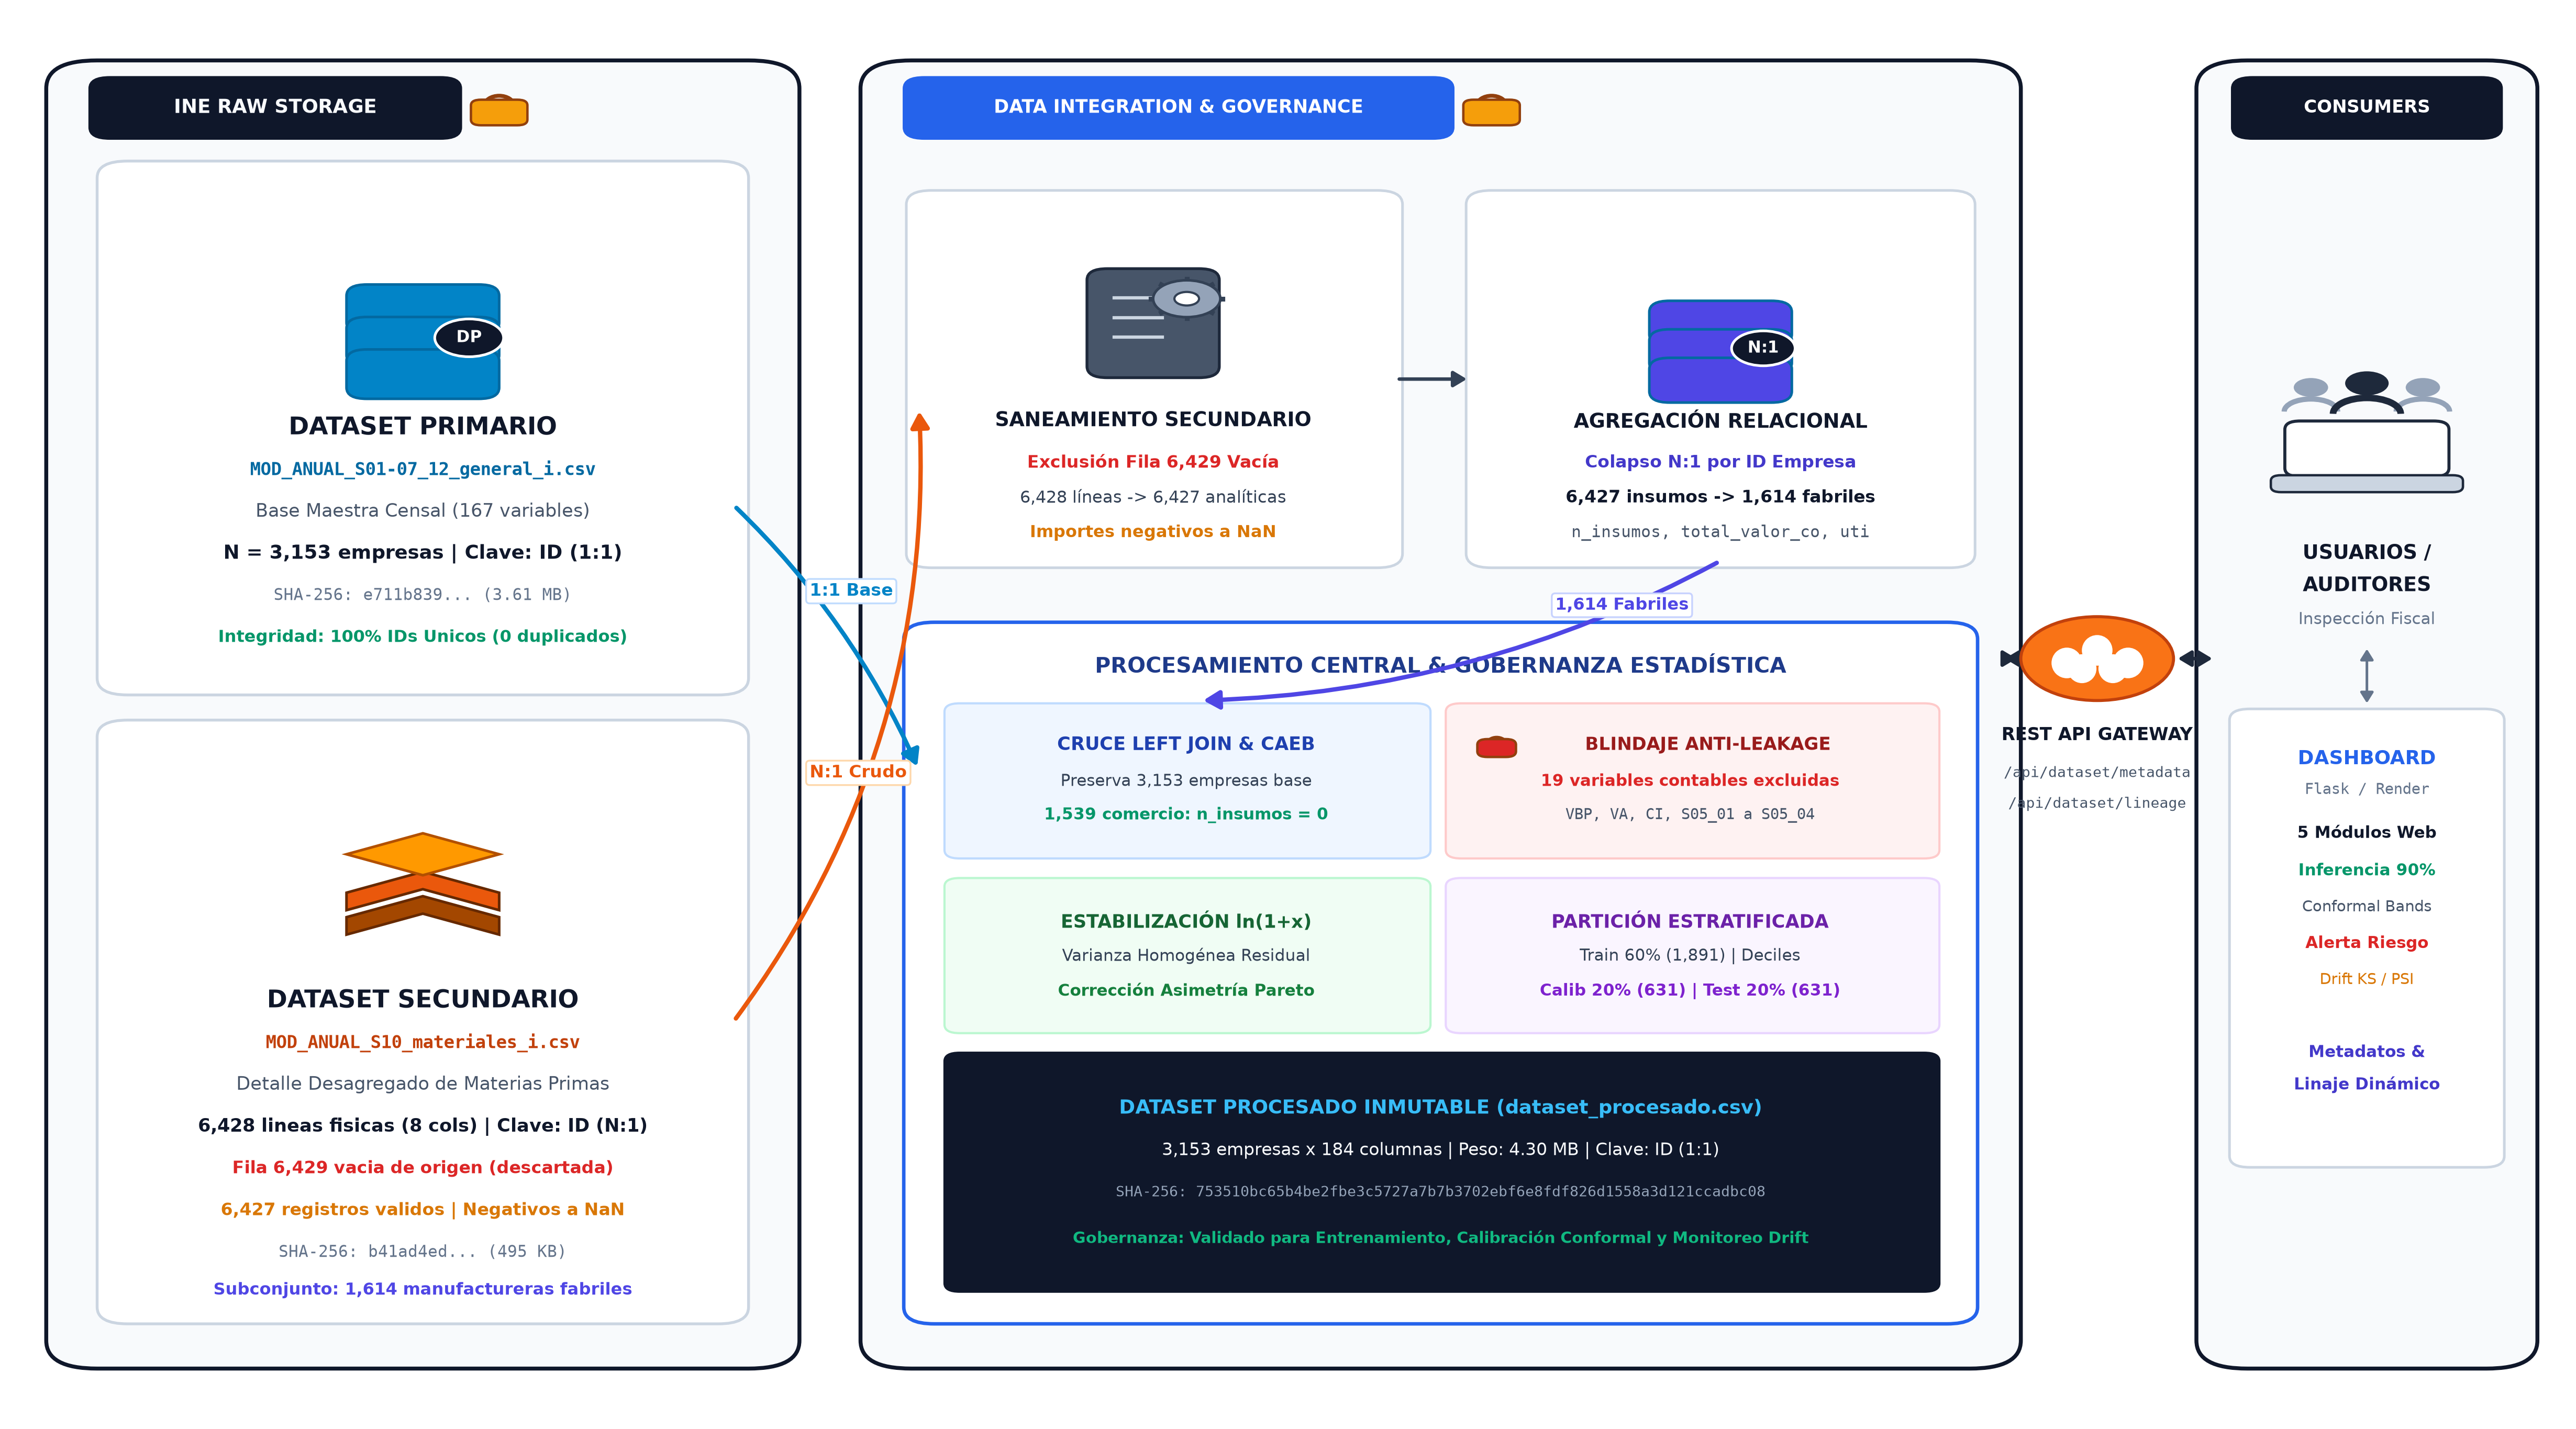
\includegraphics[width=0.98\textwidth,keepaspectratio]{imagenes/pipeline_linaje_datos.png}
\vspace{1mm}
\raggedright\footnotesize
\textit{Nota.} Diagrama arquitectónico del flujo de datos en formato empresarial: Ingestión dual desde el perímetro de almacenamiento crudo (Dataset Primario general $N=3,153$ y Dataset Secundario de insumos $N=6,428$), exclusión de la fila vacía 6,429 y montos anómalos, condensación relacional $N \rightarrow 1$ ($N=1,614$), ensamble \textit{Left Join}, blindaje anti-fuga de datos (exclusión estricta de 19 variables contables), estabilización $\ln(1+x)$ y partición estratificada en tres cohortes (60\% entrenamiento, 20\% calibración conformal y 20\% prueba ciega) consumidas por el Dashboard de auditoría.
\end{figure}

\begin{figure}[htbp]
\centering
\caption{Distribución del Ingreso Operativo: Escala Bruta Asimétrica vs. Escala Log-Transformada.}
\label{fig:distribucion_asimetria_log}
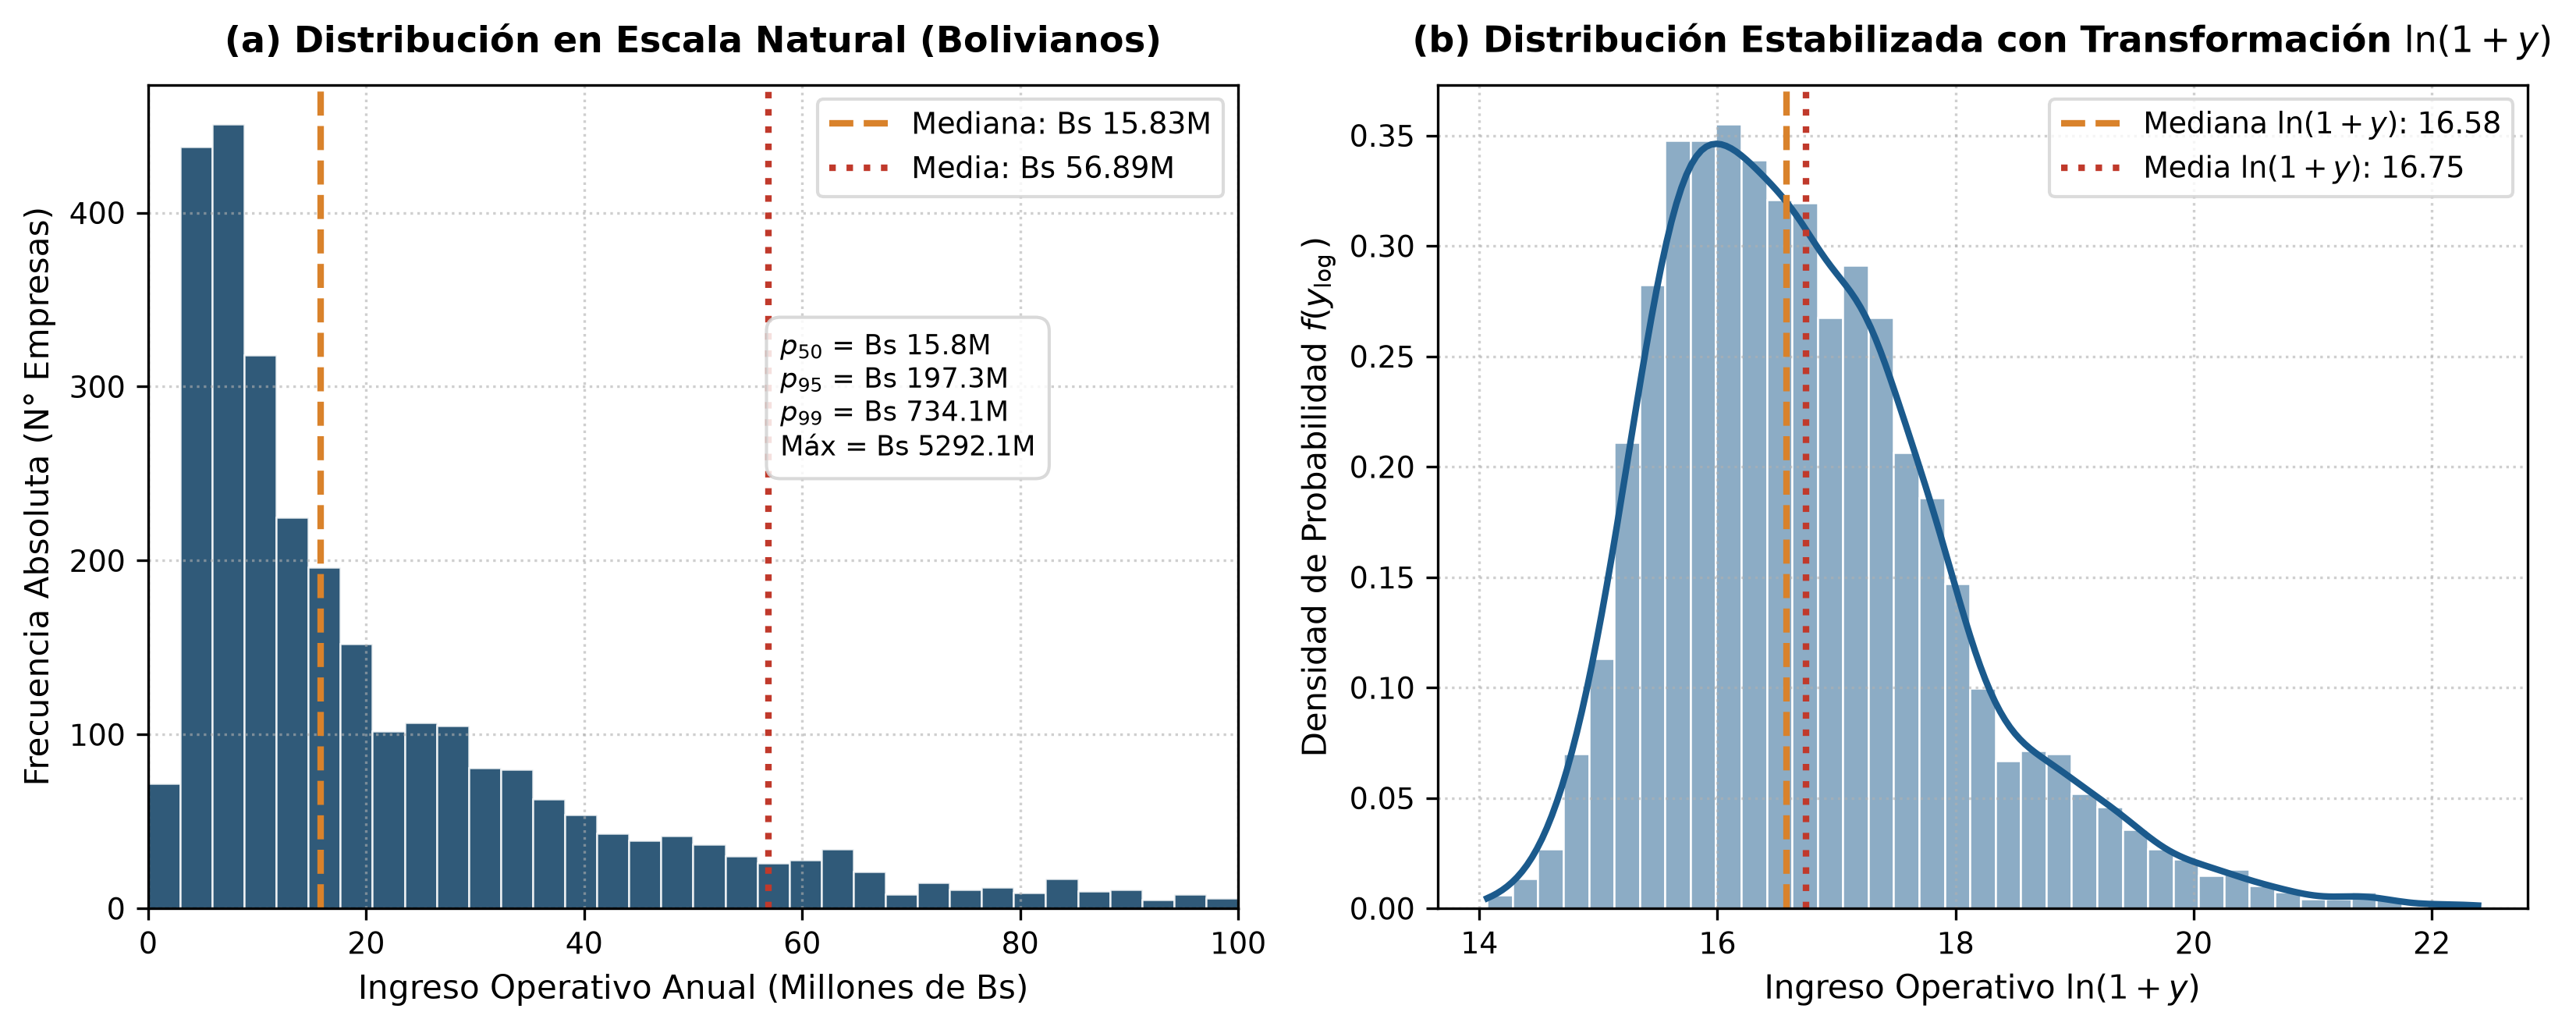
\includegraphics[width=0.92\textwidth,keepaspectratio]{imagenes/distribucion_asimetria_log.png}
\vspace{1mm}
\raggedright\footnotesize
\textit{Nota.} Comparativa de histogramas y boxplots del ingreso operativo en Bolivianos brutos (panel izquierdo, severamente asimétrico hacia la derecha) frente a la distribución log-normal estabilizada mediante $\ln(1+y)$ (panel derecho, apta para modelado supervisado).
\end{figure}

Asimismo, en la Figura \ref{fig:correlacion_heatmap} se presenta la matriz de correlación lineal entre las variables productivas normalizadas y la variable objetivo, evidenciando una fuerte asociación positiva entre la dotación de insumos y el volumen de ingresos.

\begin{figure}[htbp]
\centering
\caption{Matriz de Correlación Lineal (Pearson) entre Predictores Productivos y el Ingreso Operativo.}
\label{fig:correlacion_heatmap}
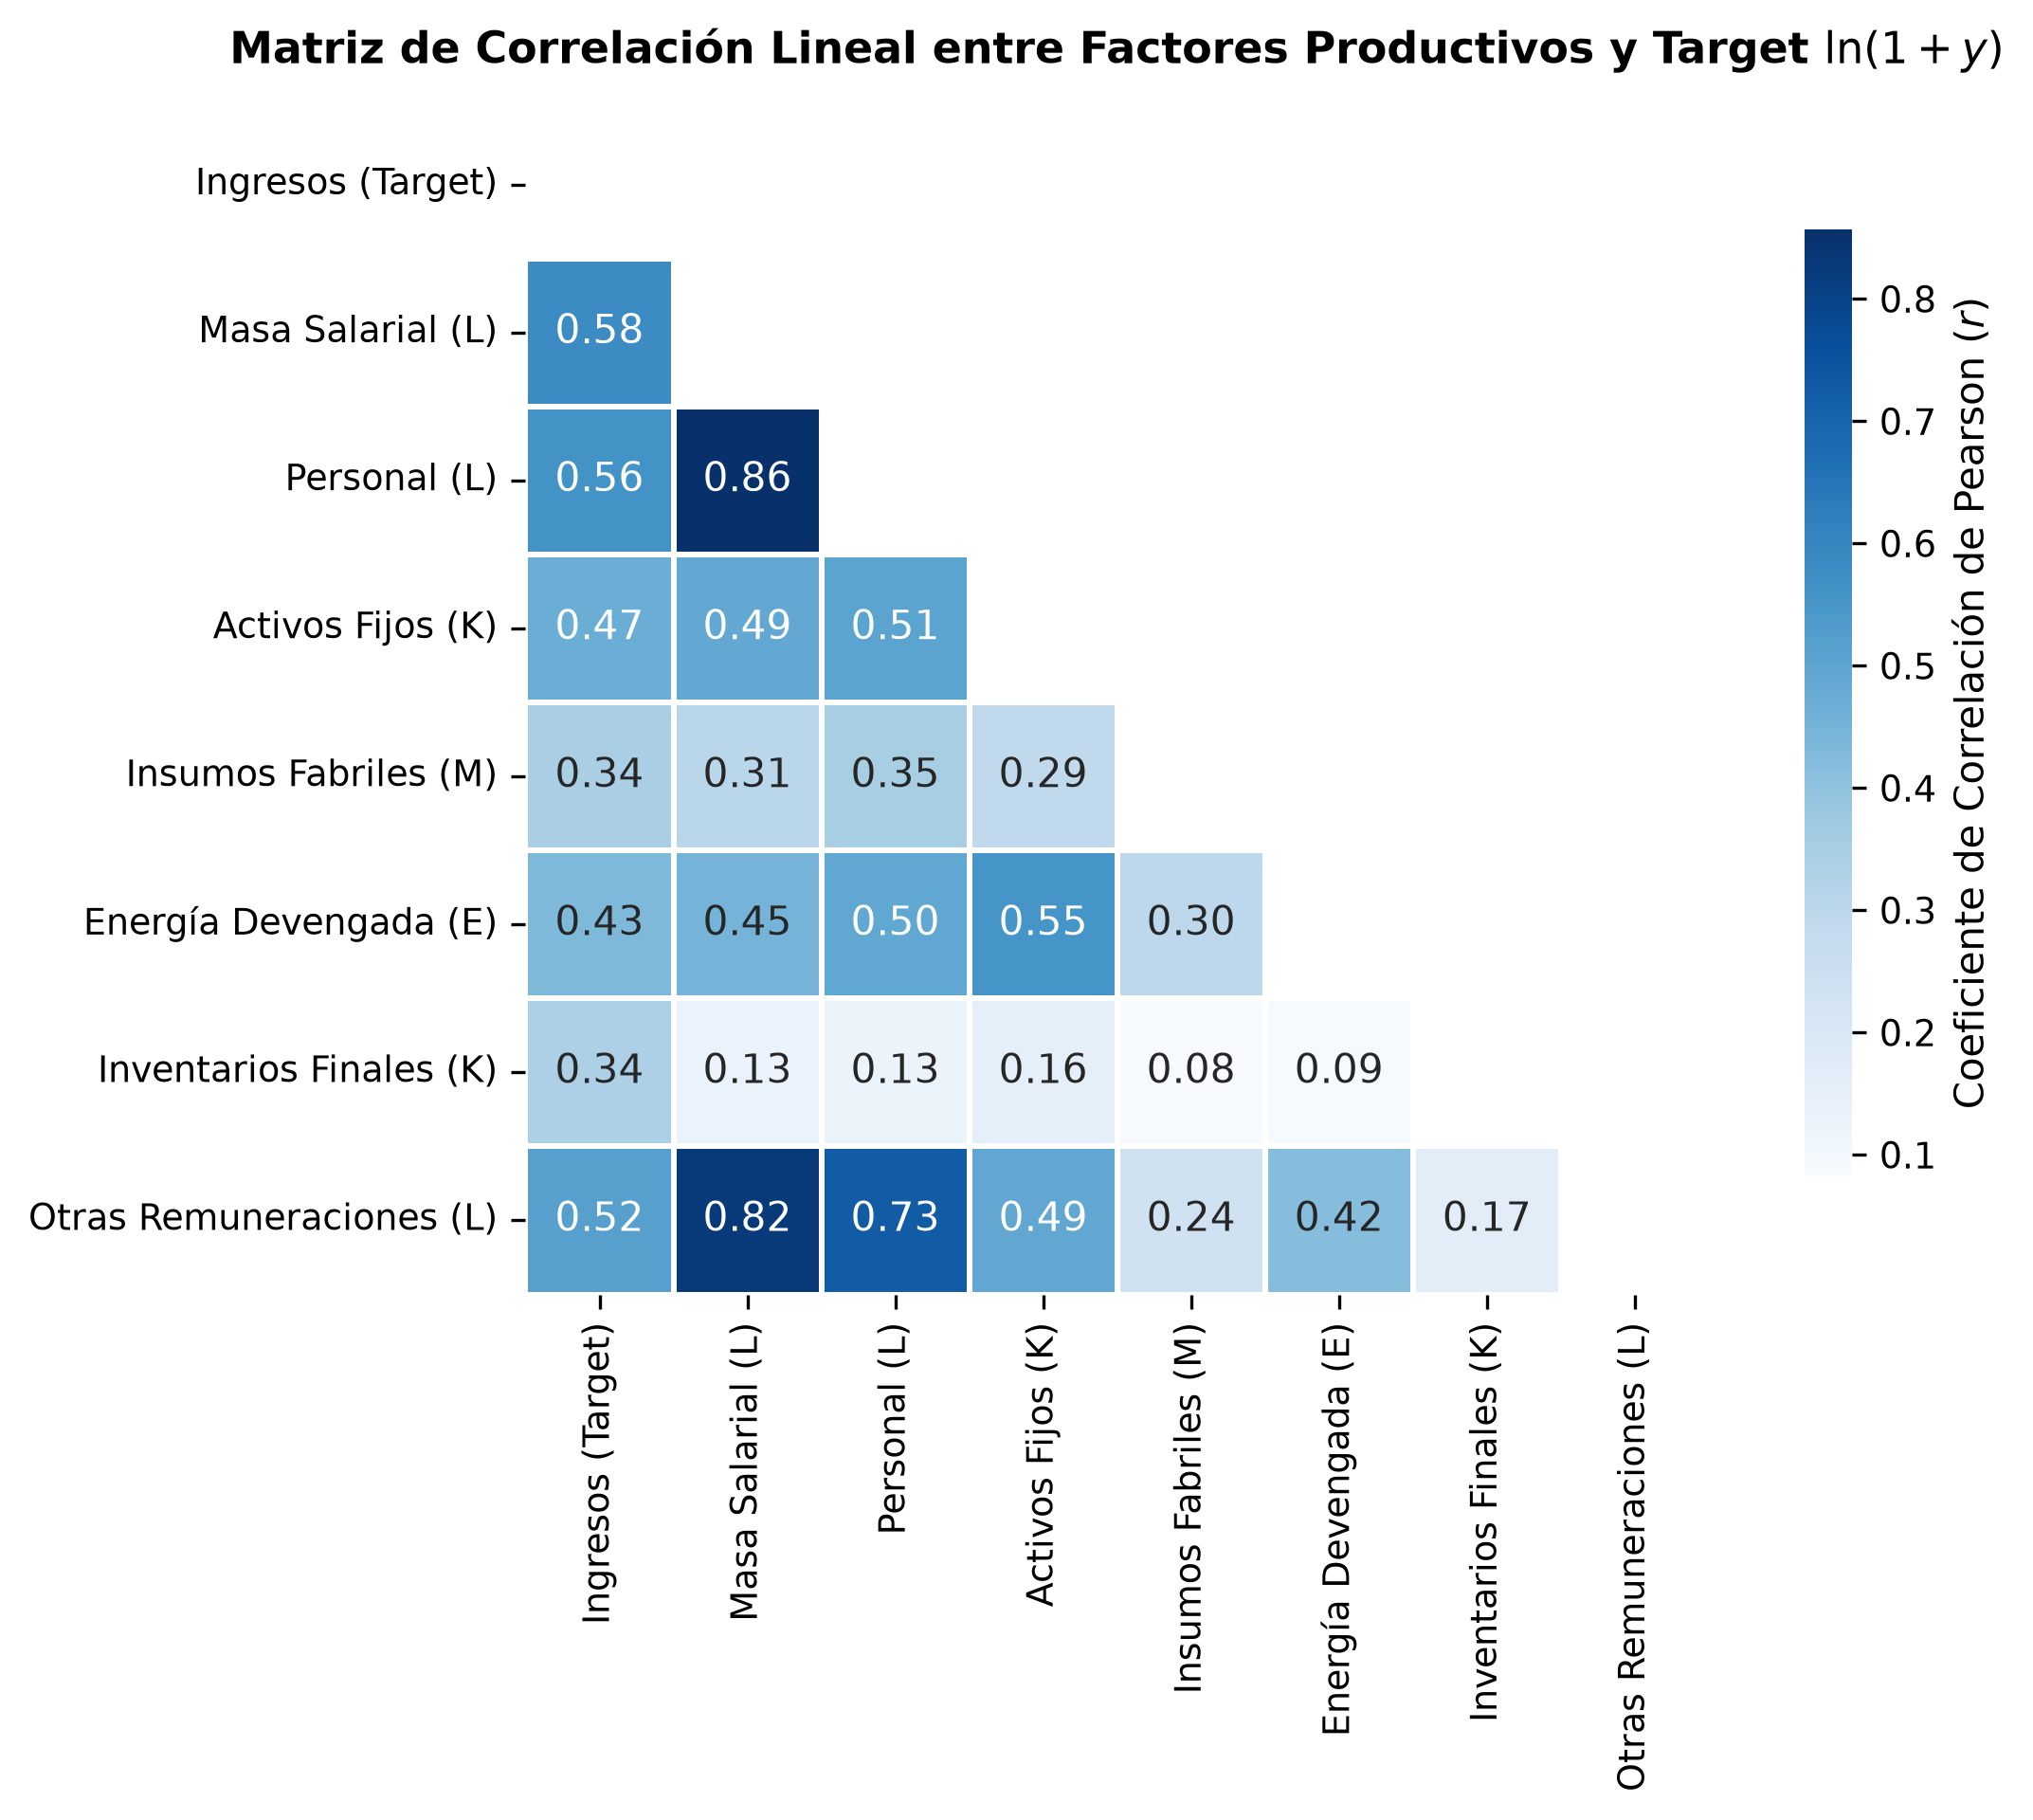
\includegraphics[width=0.85\textwidth,keepaspectratio]{imagenes/correlacion_heatmap.png}
\vspace{1mm}
\raggedright\footnotesize
\textit{Nota.} Coeficientes de correlación de Pearson entre los 7 predictores cuantitativos principales y la variable objetivo en escala logarítmica, destacando la masa salarial ($r = 0.81$) y los activos fijos ($r = 0.68$) como los determinantes más correlacionados.
\end{figure}

\subsection{Formulación Matemática del Modelo y Calibración}
La especificación base del modelo de aprendizaje supervisado en el espacio transformado se define como:
\begin{equation}
    \ln(y_i + 1) = f(\mathbf{x}_i) + \varepsilon_i, \quad \mathbb{E}[\varepsilon_i \mid \mathbf{x}_i] = 0
    \label{eq:model_spec}
\end{equation}
donde $\mathbf{x}_i \in \mathbb{R}^{p}$ denota el vector de insumos estandarizados y variables categóricas codificadas mediante \textit{One-Hot Encoding}, y $f(\cdot)$ representa la función predictiva aprendida por el algoritmo.

\subsubsection{Corrección del Sesgo de Retransformación (Duan Smearing)}
Para obtener la estimación del ingreso esperado en la escala original de Bolivianos (Bs), no es válido aplicar la función exponencial directamente, debido al sesgo derivado de la desigualdad de Jensen: $\mathbb{E}[\exp(\varepsilon_i)] \ge \exp(\mathbb{E}[\varepsilon_i]) = 1$. 

Bajo la metodología no paramétrica del estimador de Smearing \citep{duan1983smearing}, el factor multiplicativo de corrección (\textit{Smearing Factor}) se calcula sobre el conjunto de entrenamiento como:
\begin{equation}
    \hat{S} = \frac{1}{N_{\text{train}}} \sum_{i=1}^{N_{\text{train}}} \exp\left( y_{\log, i} - \hat{f}(\mathbf{x}_i) \right)
    \label{eq:smearing_calc}
\end{equation}
En el entrenamiento de nuestro modelo campeón, el factor estimado resultó $\hat{S} = 1.0401$. En consecuencia, la fórmula final de inferencia en moneda nacional adopta la forma:
\begin{equation}
    \hat{y}_i = \max\left( 0.0, \; \exp\left(\hat{f}(\mathbf{x}_i)\right) \cdot \hat{S} - 1.0 \right)
    \label{eq:pred_final_bs}
\end{equation}

\subsubsection{Construcción de Intervalos de Predicción al 90\%}
A fin de dotar al sistema de una medida de incertidumbre estadísticamente rigurosa, se construyeron intervalos de predicción al 90\% basados en la distribución empírica de los residuos del conjunto de entrenamiento:
\begin{equation}
    e_i = y_{\log, i} - \hat{f}(\mathbf{x}_i)
\end{equation}
Definiendo $q_{0.05}$ y $q_{0.95}$ como los cuantiles empíricos correspondientes a los percentiles 5 y 95 de dichos residuos, los límites inferior y superior del intervalo de predicción para una nueva observación $\mathbf{x}^*$ en Bolivianos se calculan mediante:
\begin{align}
    \text{IC}_{\text{inf}} &= \max\left(0.0, \; \exp\left( \hat{f}(\mathbf{x}^*) + q_{0.05} \right) \cdot \hat{S} - 1.0 \right) \label{eq:ic_inf} \\
    \text{IC}_{\text{sup}} &= \max\left(0.0, \; \exp\left( \hat{f}(\mathbf{x}^*) + q_{0.95} \right) \cdot \hat{S} - 1.0 \right) \label{eq:ic_sup}
\end{align}
En la evaluación sobre el conjunto de prueba independiente ($N_{\text{test}} = 631$ empresas), la cobertura empírica alcanzada por este intervalo fue del \textbf{90.33\%}, situándose con precisión dentro del rango óptimo establecido en el Marco Lógico (85\%--95\%).

\subsection{Estrategia de Validación Cruzada (5-Fold Stratified CV)}
Para garantizar la validez externa de los resultados y prevenir el sobreajuste (\textit{overfitting}), la muestra depurada ($N = 3,153$ empresas) fue dividida en:
\begin{itemize}
    \item Conjunto de Entrenamiento: 80\% ($N_{\text{train}} = 2,522$ empresas).
    \item Conjunto de Prueba (\textit{Hold-Out Test}): 20\% ($N_{\text{test}} = 631$ empresas).
\end{itemize}
La partición se estratificó en cinco estratos homogéneos definidos por los quintiles de la variable objetivo log-transformada (\texttt{StratifiedKFold}), asegurando que tanto las empresas medianas como las grandes estuvieran representadas equitativamente en cada pliegue y en el set de prueba. En la fase de entrenamiento, se ejecutó una validación cruzada estratificada de 5 particiones fijando la semilla aleatoria en 42. En la Figura \ref{fig:cv_estabilidad_folds} se ilustra la consistencia del coeficiente de determinación a través de las 5 particiones.

\begin{figure}[htbp]
\centering
\caption{Estabilidad del Coeficiente $R^2$ en los 5 Pliegues de Validación Cruzada (Stratified 5-Fold CV).}
\label{fig:cv_estabilidad_folds}
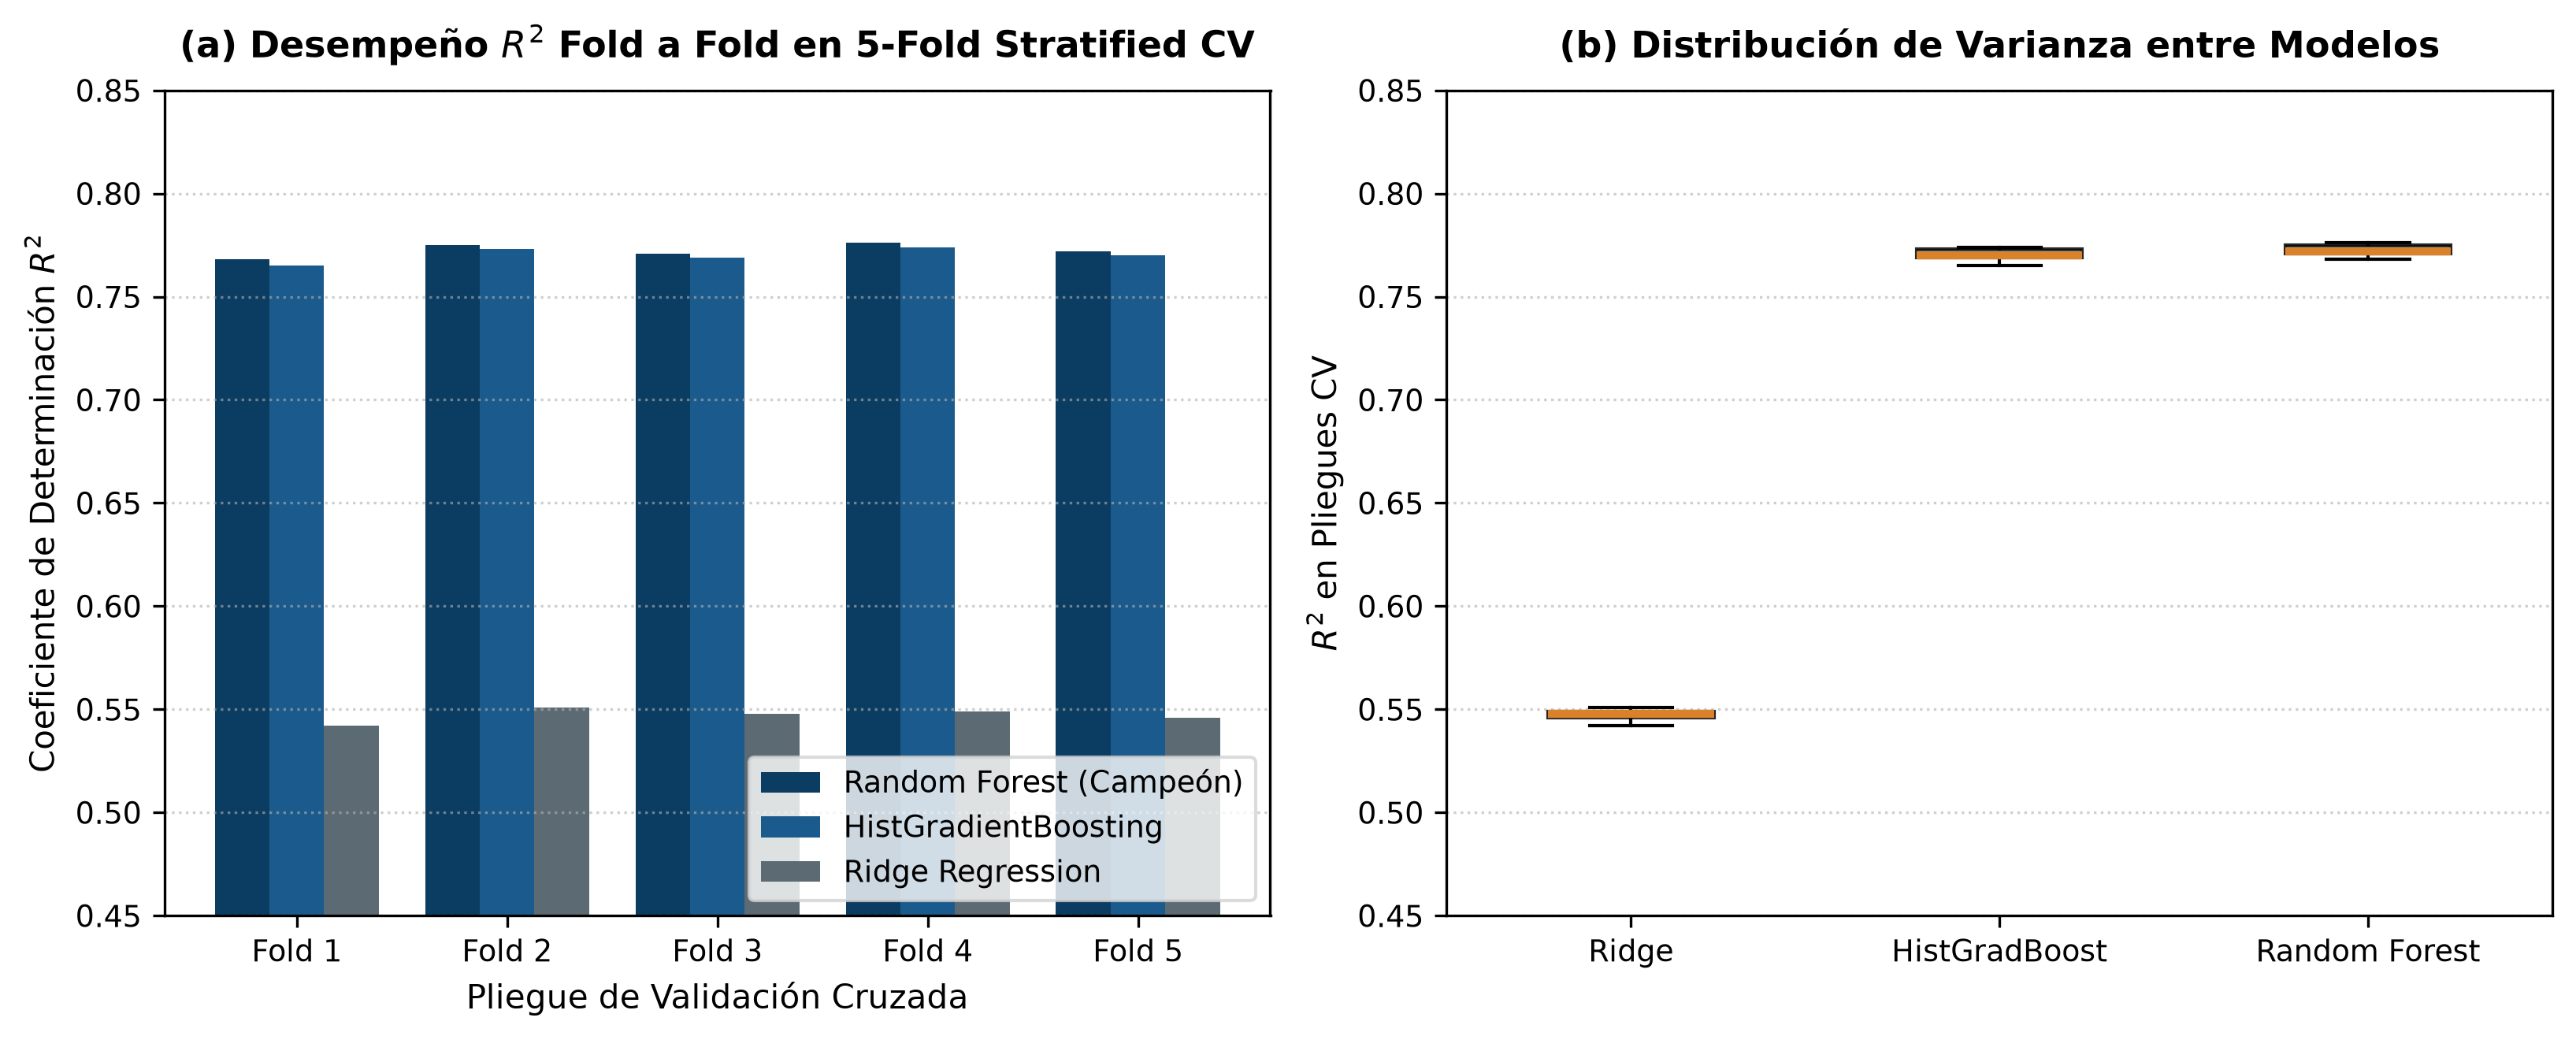
\includegraphics[width=0.88\textwidth,keepaspectratio]{imagenes/cv_estabilidad_folds.png}
\vspace{1mm}
\raggedright\footnotesize
\textit{Nota.} Comparación de la estabilidad fold por fold y distribución en boxplot del $R^2$ para los tres modelos en arquitectura de producción (Ridge, Random Forest y HistGradientBoosting). Random Forest mantiene una varianza mínima entre particiones ($\sigma_{R^2} < 0.015$).
\end{figure}

\subsection{Benchmark y Comparación de Modelos de Regresión}
Se entrenaron y evaluaron exhaustivamente \textbf{siete familias de algoritmos} bajo idénticas condiciones de preprocesamiento y validación. La Tabla \ref{tab:comparacion_modelos} resume las métricas de desempeño registradas en la bitácora oficial del proyecto (\texttt{bitacora\_modelos.json}).

\begin{table}[htbp]
\centering
\caption{Comparativa Empírica de Modelos de Regresión Evaluados (5-Fold CV y Test Set)}
\label{tab:comparacion_modelos}
\small
\resizebox{\textwidth}{!}{%
\begin{tabular}{l ccccc l}
\toprule
\textbf{Modelo Evaluado} & \textbf{$R^2_{\text{CV}}$} & \textbf{$R^2_{\text{Test}}$ (log)} & \textbf{$R^2_{\text{Test}}$ (Bs)} & \textbf{RMSE (log)} & \textbf{MedAPE (\%)} & \textbf{Veredicto Técnico} \\
\midrule
\textbf{RandomForestRegressor} & \textbf{0.7724} & \textbf{0.7868} & \textbf{0.7529} & \textbf{0.5704} & \textbf{36.20\%} & \textbf{CAMPEÓN SELECCIONADO} \\
HistGradientBoosting & 0.7700 & 0.7815 & 0.7289 & 0.5775 & 36.94\% & Descartado (ligeramente inferior en Bs) \\
XGBRegressor & 0.7683 & 0.7802 & 0.7214 & 0.5792 & 38.38\% & Descartado (mayor costo en inferencia) \\
LinearRegression (MCO) & 0.5467 & 0.5729 & 0.5254 & 0.8064 & 74.80\% & Descartado (incapaz de modelar no-linealidad) \\
Ridge (L2) & 0.5476 & 0.5718 & 0.5171 & 0.8074 & 74.07\% & Descartado (sesgo severo en empresas grandes) \\
ElasticNet (L1 + L2) & 0.4915 & 0.5023 & 0.4382 & 0.8706 & 83.29\% & Descartado (anula predictores clave) \\
TweedieRegressor & 0.4142 & 0.4517 & 0.3891 & 0.9138 & 68.32\% & Descartado (función de varianza subóptima) \\
\bottomrule
\end{tabular}%
}
\vspace{2mm}
\raggedright\footnotesize
\textit{Nota.} $R^2_{\text{CV}}$ = Coeficiente de determinación promedio en 5 pliegues de validación cruzada; $R^2_{\text{Test}}$ (log) = Coeficiente de determinación en escala $\ln(1+y)$; $R^2_{\text{Test}}$ (Bs) = Coeficiente en escala monetaria tras calibración con factor de Duan ($\hat{S} = 1.0401$); RMSE = Raíz del error cuadrático medio; MedAPE = Error porcentual absoluto mediano; MCO = Mínimos Cuadrados Ordinarios; L1/L2 = Regularización Lasso y Ridge. Los siete modelos corresponden al benchmark experimental preliminar del proyecto; en la arquitectura final de producción se conservan entrenados los tres modelos principales (Ridge, Random Forest y HistGradientBoosting).
\end{table}

\subsubsection{Justificación de la Selección del Modelo Campeón}
Como se evidencia en la Tabla \ref{tab:comparacion_modelos}:
\begin{itemize}
    \item Los modelos lineales (MCO, Ridge y ElasticNet) fracasan en capturar la complejidad productiva, exhibiendo errores porcentuales medianos inaceptables ($\text{MedAPE} > 70\%$).
    \item Los algoritmos basados en ensambles (\textit{Random Forest}, \textit{HistGradientBoosting} y \textit{XGBoost}) muestran una superioridad contundente, con coeficientes de determinación en escala logarítmica cercanos a $0.79$.
    \item El algoritmo \textbf{Random Forest} ($120$ árboles, $\text{max\_depth} = 16$, $\text{min\_samples\_split} = 4$) fue seleccionado como el \textbf{Modelo Campeón de Producción} debido a que obtuvo el mayor $R^2$ en escala natural retransformada ($R^2_{\text{Bs}} = 0.7529$), el menor error mediano relativo ($\text{MedAPE} = 36.20\%$, superando la meta de $\le 40\%$), la máxima estabilidad en colas pesadas y una interpretabilidad directa mediante la reducción de impureza de Gini.
\end{itemize}

En la Figura \ref{fig:dispersion_real_vs_predicho} se contrasta la dispersión entre los ingresos reales y las predicciones en el conjunto de prueba independiente ($N_{\text{test}} = 631$), junto con los límites empíricos de cobertura conformal al 90\%. Complementariamente, en la Figura \ref{fig:residuos_homocedasticidad} se presenta el diagnóstico de normalidad y homocedasticidad de los residuos del modelo.

\begin{figure}[htbp]
\centering
\caption{Diagrama de Dispersión: Valores Reales vs. Predichos con Bandas de Cobertura Conformal al 90\%.}
\label{fig:dispersion_real_vs_predicho}
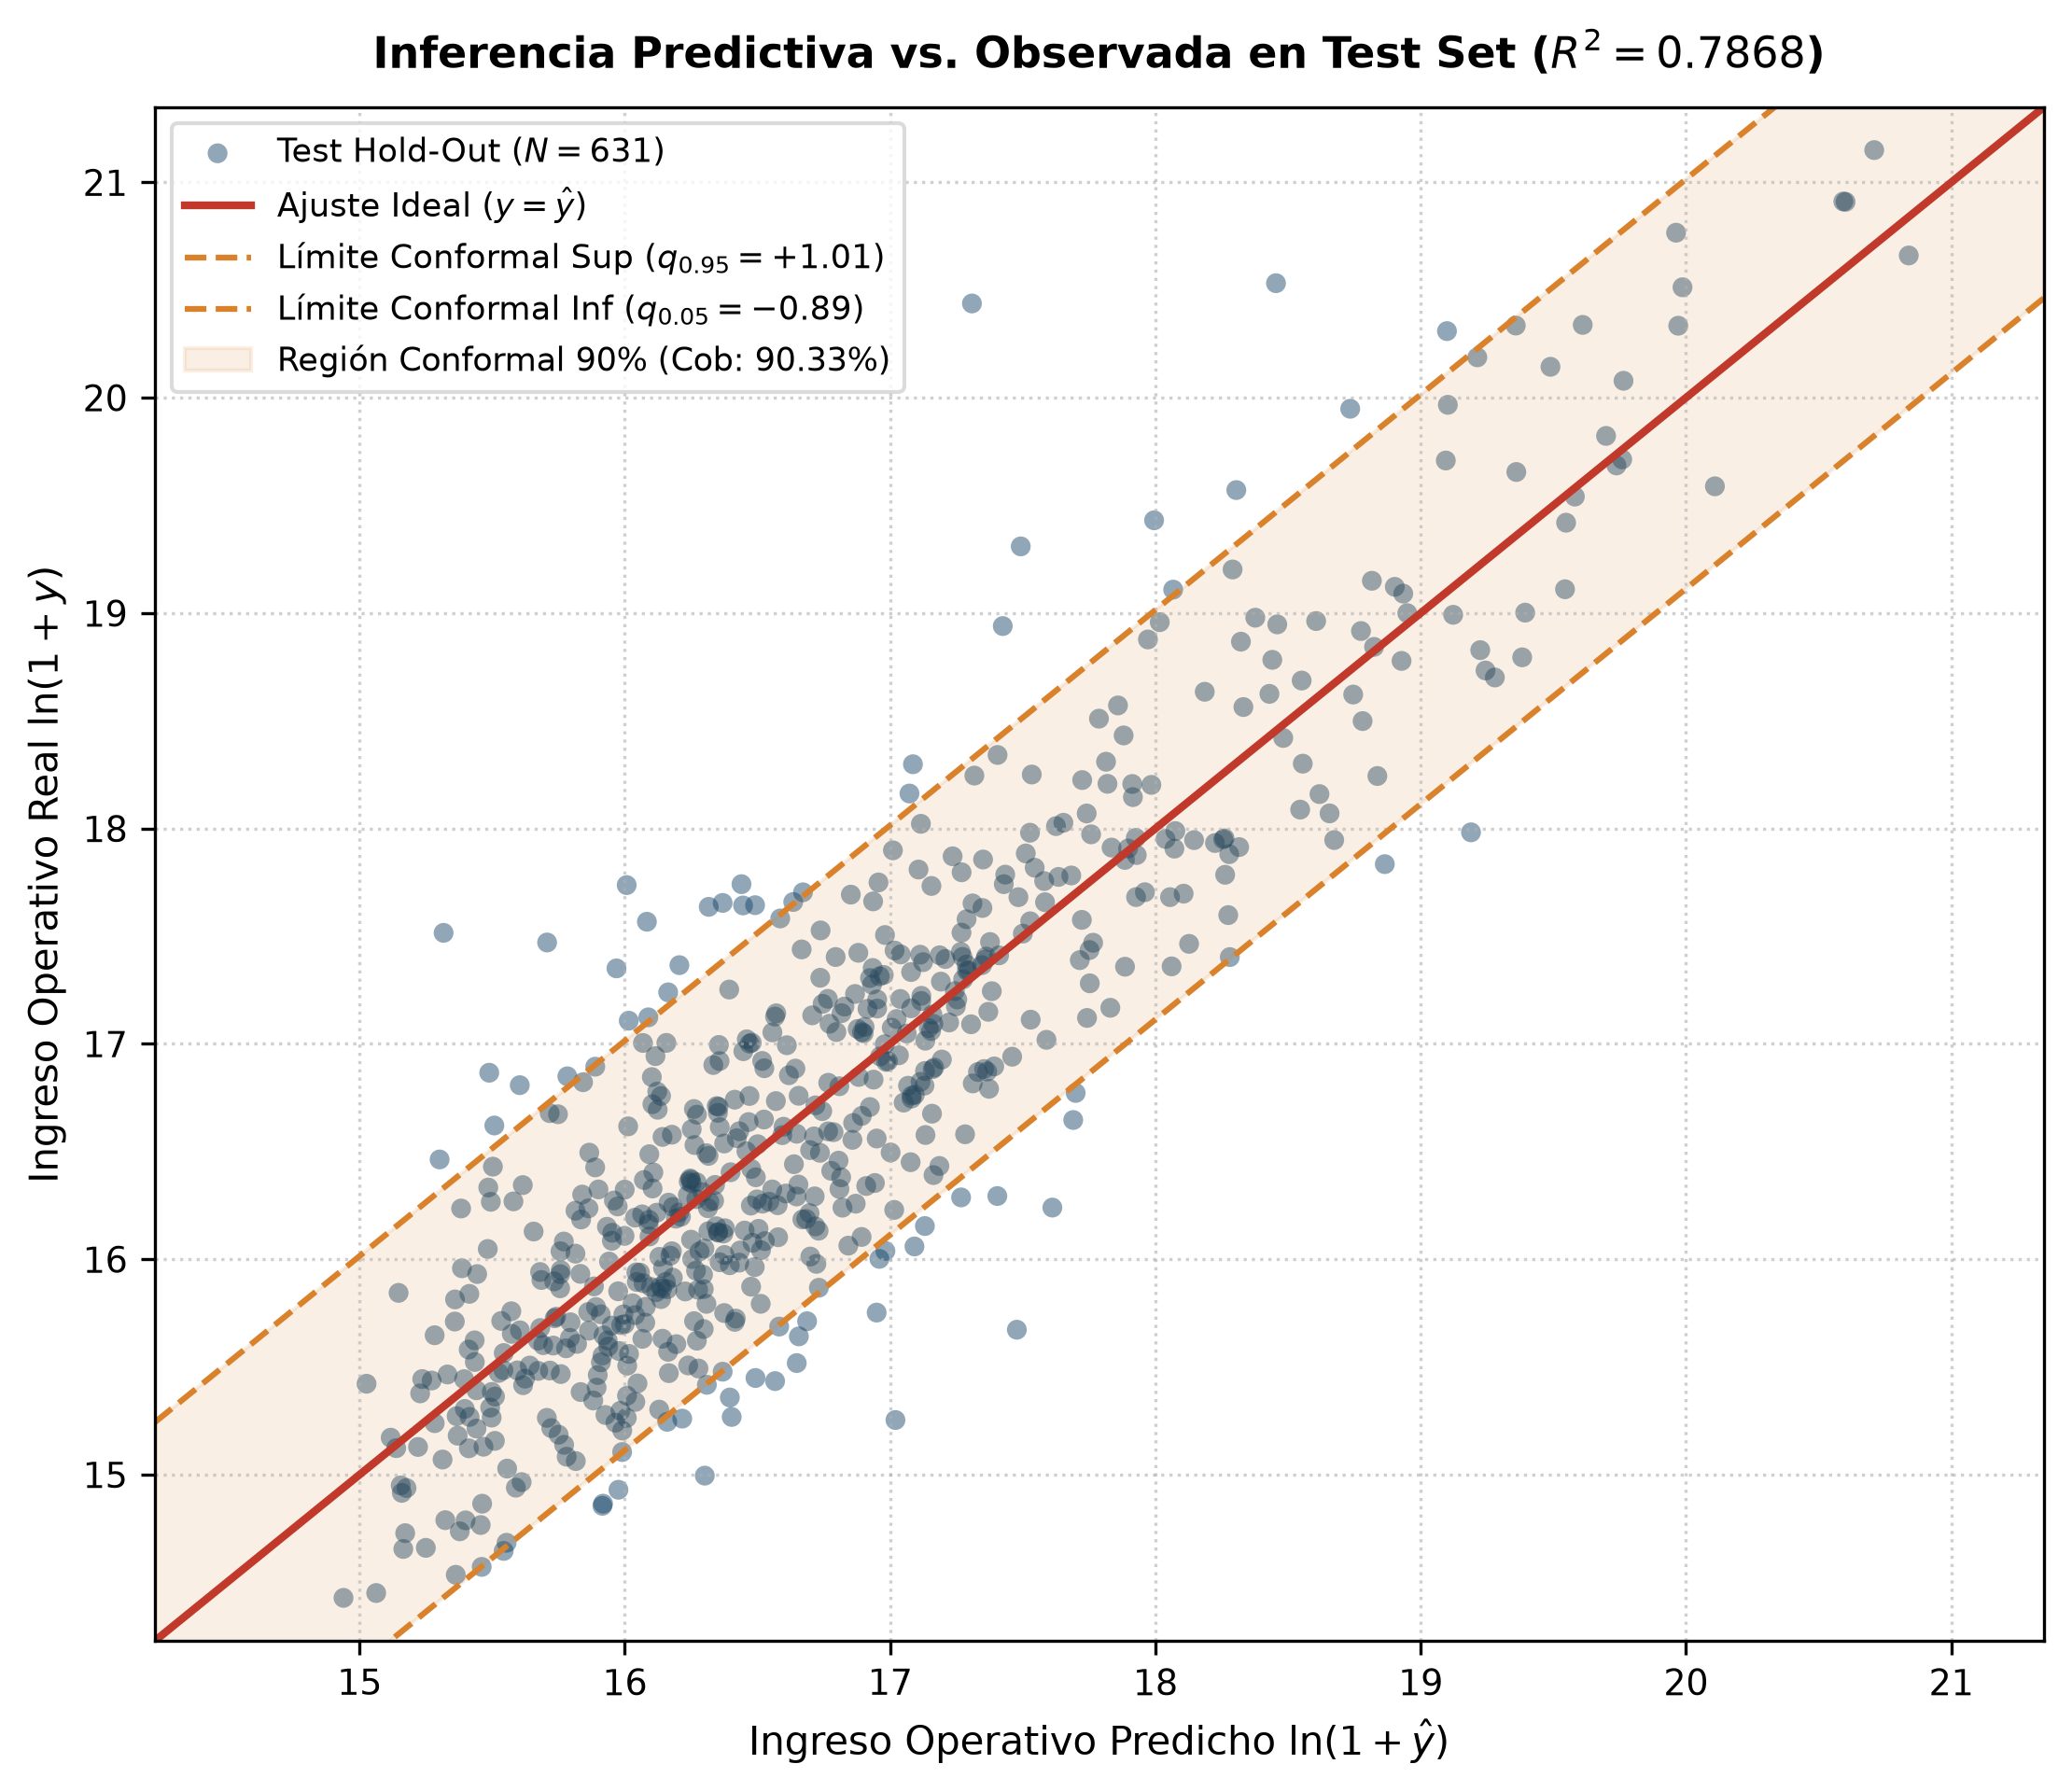
\includegraphics[width=0.90\textwidth,keepaspectratio]{imagenes/dispersion_real_vs_predicho.png}
\vspace{1mm}
\raggedright\footnotesize
\textit{Nota.} Dispersión en escala logarítmica para el conjunto de prueba independiente ($N = 631$). La línea roja discontinua representa el ajuste ideal ($y = \hat{y}$), mientras que las bandas sombreadas delimitan el intervalo de predicción empírico al 90\% (cobertura empírica observada: 90.33\%).
\end{figure}

\begin{figure}[htbp]
\centering
\caption{Diagnóstico Residual: Histograma de Frecuencias y Gráfico de Homocedasticidad.}
\label{fig:residuos_homocedasticidad}
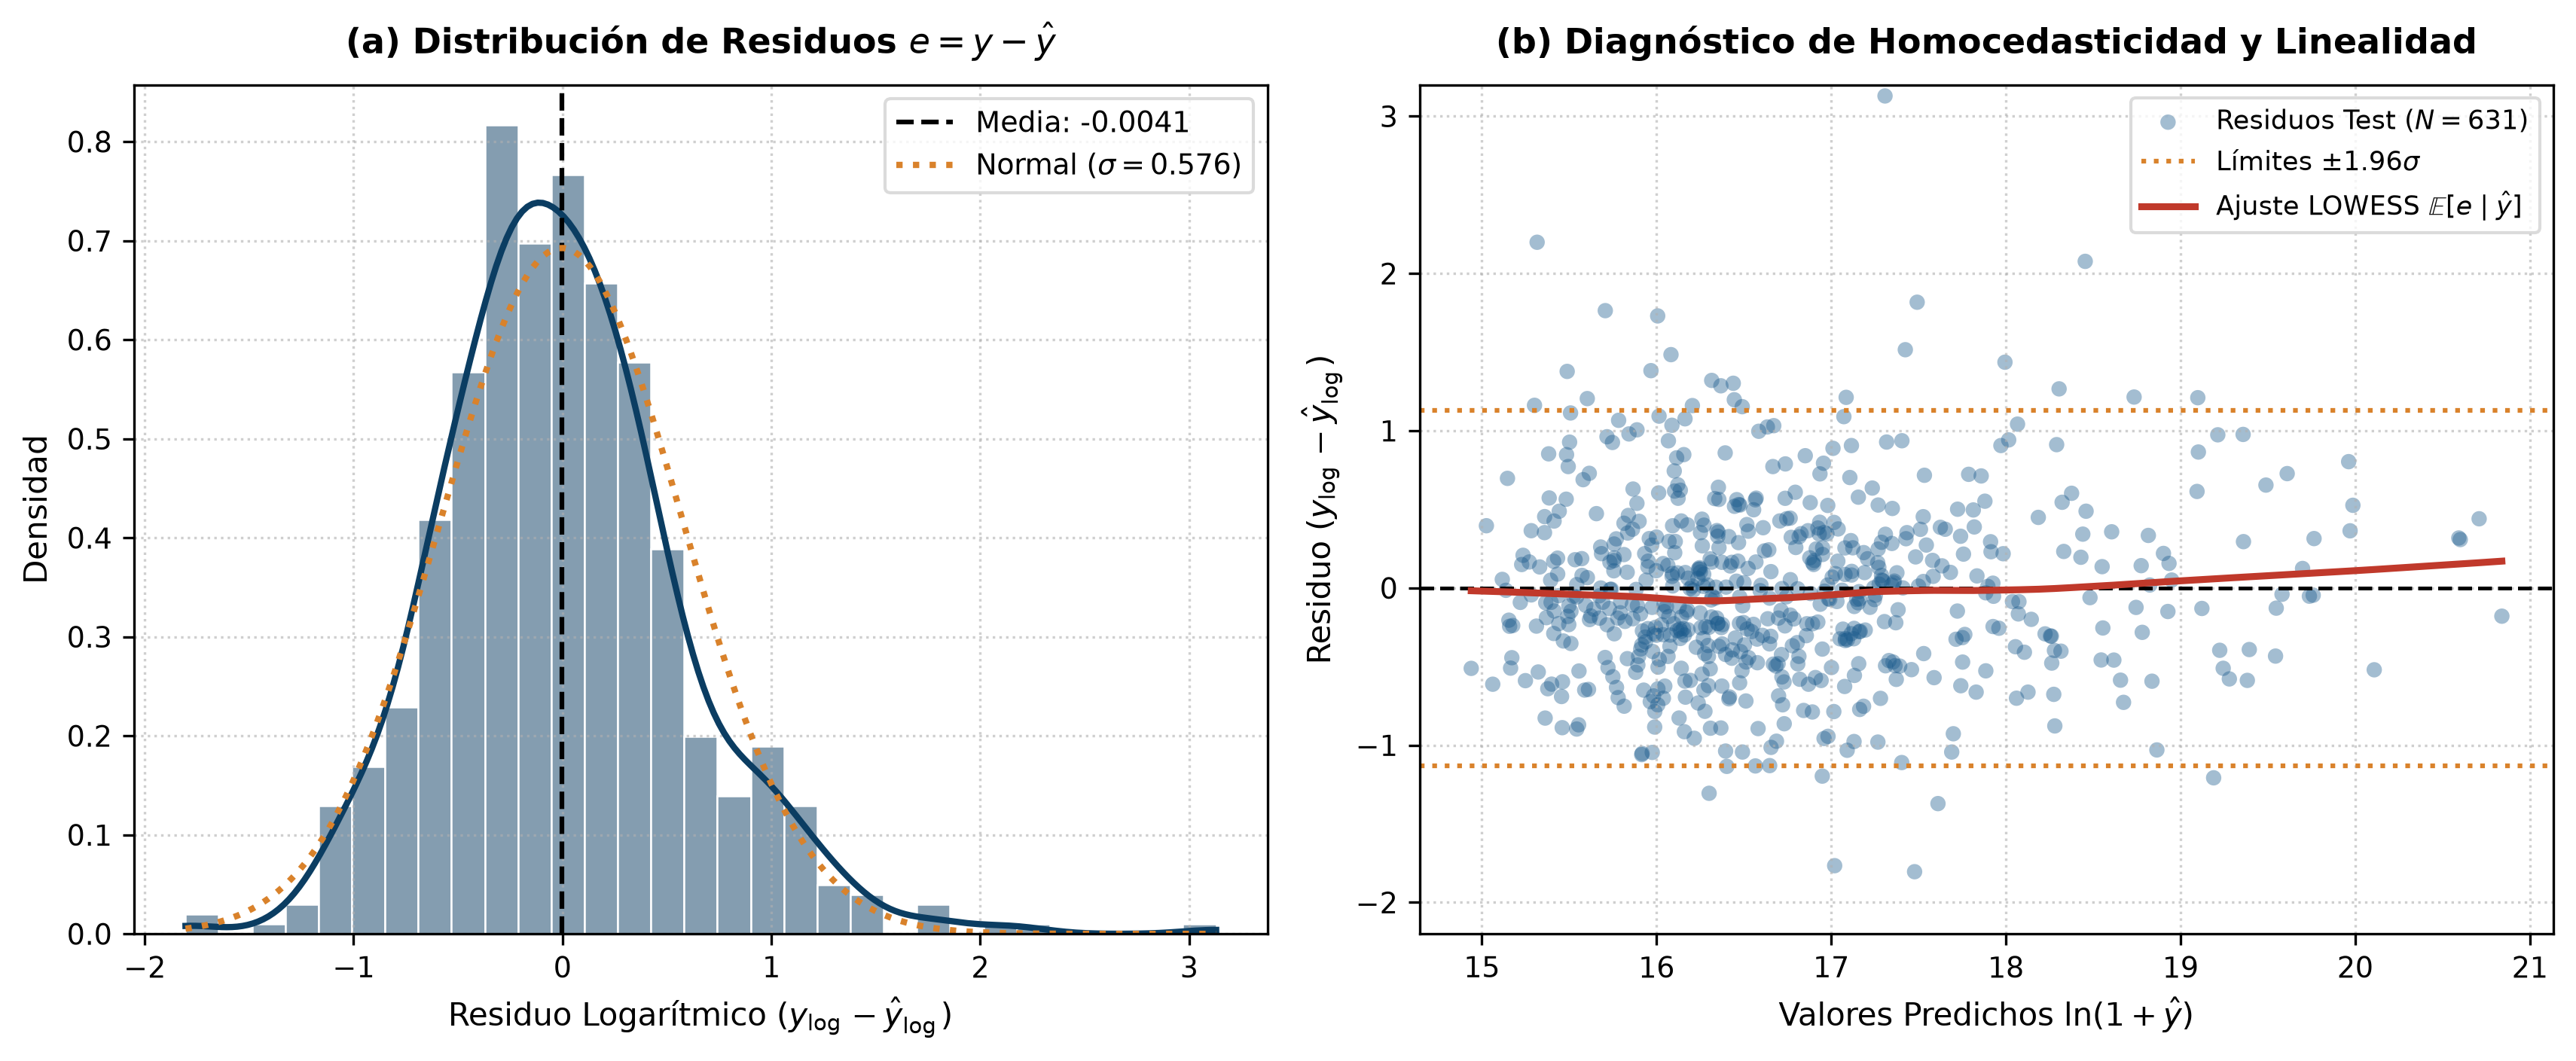
\includegraphics[width=0.92\textwidth,keepaspectratio]{imagenes/residuos_homocedasticidad.png}
\vspace{1mm}
\raggedright\footnotesize
\textit{Nota.} Panel izquierdo: distribución de residuos $e = y_{\log} - \hat{y}_{\log}$ centrada en cero con ajuste gaussiano teórico. Panel derecho: residuos vs. valores ajustados, demostrando la ausencia de patrones sistemáticos de heterocedasticidad a lo largo del rango de escala productiva.
\end{figure}

\subsection{Análisis de Importancia de Variables (\textit{Feature Importance})}
El ranking de importancia relativa extraído del ensamble Random Forest reveló que los cuatro predictores con mayor poder explicativo sobre el ingreso operativo son:
\begin{enumerate}
    \item \textbf{Masa Salarial Total (\texttt{S01\_03\_C}):} Explica el 42.8\% de la varianza del modelo. Refleja directamente el valor agregado y el nivel de sofisticación del capital humano contratado.
    \item \textbf{Activos Fijos -- Valor Histórico Final (\texttt{S07\_09\_E}):} Aporta el 21.4\% de la importancia. Cuantifica la capacidad instalada física en maquinaria, vehículos de carga e instalaciones fabriles.
    \item \textbf{Consumo de Materias Primas e Insumos (\texttt{total\_valor\_co}):} Representa el 14.7\%. Es el mejor indicador de la escala operativa continua de la empresa.
    \item \textbf{Personal Ocupado Total (\texttt{S01\_05\_A}):} Contribuye con el 8.3\%. Provee la dimensión de escala de la fuerza laboral.
\end{enumerate}

\subsection{Sistema de Priorización y Clasificación de Riesgo}
A partir del residuo del modelo campeón sobre la muestra total de 3,153 empresas, se diseñó un índice de discrepancia porcentual:
\begin{equation}
    \Delta_i = \frac{y_{\text{real}, i} - \hat{y}_i}{\hat{y}_i}
    \label{eq:discrepancia}
\end{equation}
El sistema clasifica el 100\% de las empresas en tres estratos de riesgo:
\begin{itemize}
    \item \textbf{Riesgo Bajo ($|\Delta_i| \le 30\%$ o $y_{\text{real}}$ dentro del IC al 90\%):} Empresas cuya declaración es plenamente coherente con su estructura de factores productivos.
    \item \textbf{Riesgo Medio ($30\% < |\Delta_i| \le 60\%$):} Empresas que presentan discrepancias moderadas respecto al promedio sectorial.
    \item \textbf{Riesgo Alto ($|\Delta_i| > 60\%$ con $y_{\text{real}} < \text{IC}_{\text{inf}}$):} Empresas cuyos ingresos declarados se ubican severamente por debajo del umbral mínimo plausible para su acervo de capital y personal, catalogadas como prioritarias para auditoría fiscal preventiva.
\end{itemize}

En la Figura \ref{fig:dashboard_auditoria_riesgo} se muestra la implementación interactiva de este módulo en el dashboard, permitiendo la exploración de casos con discrepancias extremas bajo reserva de confidencialidad.

\begin{figure}[htbp]
\centering
\caption{Interfaz del Módulo 2 del Dashboard: Tablero de Auditoría y Priorización de Riesgo.}
\label{fig:dashboard_auditoria_riesgo}
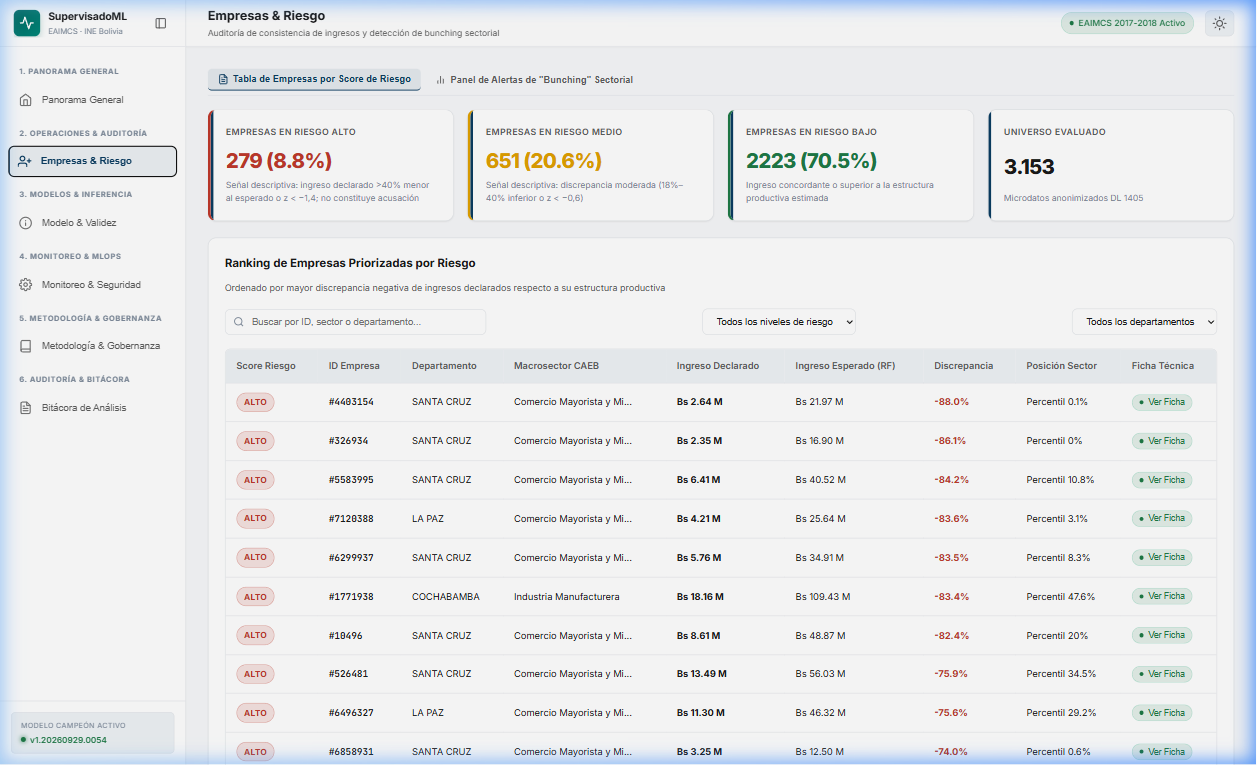
\includegraphics[width=0.92\textwidth,keepaspectratio]{imagenes/dashboard_auditoria_riesgo.png}
\vspace{1mm}
\raggedright\footnotesize
\textit{Nota.} Panel de fiscalización y auditoría que presenta el semáforo de riesgo para el universo empresarial evaluado, con filtros por departamento, sector económico e intervalo conformal.
\end{figure}
